\problemname{Reseplaneraren}

\noindent
After using public transport for several years, you have noticed that Bästtrafik's route planning app is not very good.
It often suggests routes with 3 transfers, when you know that the journey can be made without any transfers at all! To demonstrate
how incompetent they are, you will develop a competing app that determines if it is possible to travel from station $A$ to
station $B$ without any transfers.

The public transport network in Gothenburg can be described by its $N$ stations. 
These stations are connected by several roads. 
The network of roads is designed so that it is possible to travel between every pair of stations, and it contains exactly $N-1$ roads. 
This means that the road network forms a tree. 
In a tree, a path is defined as a sequence of stations where each station is directly connected to the next in the sequence, 
and no station is visited more than once. The path between two stations is always the shortest and the only possible path connecting them. 
The public transport consists of $K$ tram lines running through the network.
Each tram line has a tram that travels between two stations, start and end. This tram travels back and forth between the start
and end stations repeatedly. The roads have enough tracks to ensure that trams never get stuck or end up in a traffic jam.

Your app must now answer $Q$ questions of the form: "Can you travel from station $a$ to station $b$
without transfers?" In other words, can you board a tram at station $a$, let the tram ride for a while, and then get off at
station $b$? To mock Besttrafik as much as possible, you don't care at all about how long the journey takes.

\section*{Input}
The first line of input contains the integers $N$, $K$, and $Q$ ($1 \le N, K, Q \le 3 \cdot 10^5$), the number of stations,
tram lines, and questions.

The following $N-1$ lines each contain two integers $u,v$ ($1 \leq u,v \leq N$, $u \neq v$),
which means that there is a road between station $u$ and station $v$. 

Next, $K$ lines follow, each containing two integers $s,t$ ($1 \leq s,t \leq N$, $s \neq t$), which
means that there is a tram line between stations $s$ and $t$.

The final $Q$ lines each contain two integers $a,b$ ($1 \leq a,b \leq N$, $a \neq b$), representing a question of whether you can travel from station $a$ to station $b$ without transfers. 

\textbf{Note} that this problem has a very large input size. Therefore, it is recommended to use fast input reading.

\section*{Output}
For each question, print ``Yes'' if it is possible to make the journey without transfers, otherwise
print ``No''. Print these in the same order as the questions.

\section*{Scoring}
Your solution will be tested on a set of test groups, each worth a number of points. Each test group contains
a set of test cases. To get the points for a test group you need to solve all test cases in the test group.

\noindent
\begin{tabular}{| l | l | p{12cm} |}
  \hline
  \textbf{Group} & \textbf{Points} & \textbf{Constraints} \\ \hline
  $1$    & $2$        & $N \leq 10$ \\ \hline
  $2$    & $15$       & $N \leq 40$ \\ \hline
  $3$    & $30$       & $N \leq 1000$ \\ \hline
  $4$    & $53$       & No additional constraints. \\ \hline
\end{tabular}

\section*{Explanation of Sample 1}
\begin{figure}[h]
  \centering
  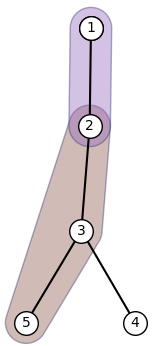
\includegraphics{sample.png}
  \caption{Visualization of Sample 1. The black edges represent the roads, and the colored areas represent each tram line.}
  \label{fig:example1}
\end{figure}

\begin{itemize}
  \item Question 1: It is not possible to travel from station 1 to station 3 without a transfer. If transferring once were allowed, it would have been possible.
  \item Question 2: There isn't even a tram line going to station 4, so it is certainly not possible to make the journey without transfers.
  \item Question 3: Here, we can take the tram line between stations 1 and 2.
  \item Question 4: Here, we can take the tram line between stations 5 and 3.
\end{itemize}
